\documentclass[]{book}
\usepackage{lmodern}
\usepackage{amssymb,amsmath}
\usepackage{ifxetex,ifluatex}
\usepackage{fixltx2e} % provides \textsubscript
\ifnum 0\ifxetex 1\fi\ifluatex 1\fi=0 % if pdftex
  \usepackage[T1]{fontenc}
  \usepackage[utf8]{inputenc}
\else % if luatex or xelatex
  \ifxetex
    \usepackage{mathspec}
  \else
    \usepackage{fontspec}
  \fi
  \defaultfontfeatures{Ligatures=TeX,Scale=MatchLowercase}
\fi
% use upquote if available, for straight quotes in verbatim environments
\IfFileExists{upquote.sty}{\usepackage{upquote}}{}
% use microtype if available
\IfFileExists{microtype.sty}{%
\usepackage{microtype}
\UseMicrotypeSet[protrusion]{basicmath} % disable protrusion for tt fonts
}{}
\usepackage[margin=1in]{geometry}
\usepackage{hyperref}
\hypersetup{unicode=true,
            pdftitle={GAMA Model Documentations},
            pdfauthor={Srirama Bhamidipati, Erika S, Arend L},
            pdfborder={0 0 0},
            breaklinks=true}
\urlstyle{same}  % don't use monospace font for urls
\usepackage{natbib}
\bibliographystyle{plainnat}
\usepackage{color}
\usepackage{fancyvrb}
\newcommand{\VerbBar}{|}
\newcommand{\VERB}{\Verb[commandchars=\\\{\}]}
\DefineVerbatimEnvironment{Highlighting}{Verbatim}{commandchars=\\\{\}}
% Add ',fontsize=\small' for more characters per line
\usepackage{framed}
\definecolor{shadecolor}{RGB}{248,248,248}
\newenvironment{Shaded}{\begin{snugshade}}{\end{snugshade}}
\newcommand{\AlertTok}[1]{\textcolor[rgb]{0.94,0.16,0.16}{#1}}
\newcommand{\AnnotationTok}[1]{\textcolor[rgb]{0.56,0.35,0.01}{\textbf{\textit{#1}}}}
\newcommand{\AttributeTok}[1]{\textcolor[rgb]{0.77,0.63,0.00}{#1}}
\newcommand{\BaseNTok}[1]{\textcolor[rgb]{0.00,0.00,0.81}{#1}}
\newcommand{\BuiltInTok}[1]{#1}
\newcommand{\CharTok}[1]{\textcolor[rgb]{0.31,0.60,0.02}{#1}}
\newcommand{\CommentTok}[1]{\textcolor[rgb]{0.56,0.35,0.01}{\textit{#1}}}
\newcommand{\CommentVarTok}[1]{\textcolor[rgb]{0.56,0.35,0.01}{\textbf{\textit{#1}}}}
\newcommand{\ConstantTok}[1]{\textcolor[rgb]{0.00,0.00,0.00}{#1}}
\newcommand{\ControlFlowTok}[1]{\textcolor[rgb]{0.13,0.29,0.53}{\textbf{#1}}}
\newcommand{\DataTypeTok}[1]{\textcolor[rgb]{0.13,0.29,0.53}{#1}}
\newcommand{\DecValTok}[1]{\textcolor[rgb]{0.00,0.00,0.81}{#1}}
\newcommand{\DocumentationTok}[1]{\textcolor[rgb]{0.56,0.35,0.01}{\textbf{\textit{#1}}}}
\newcommand{\ErrorTok}[1]{\textcolor[rgb]{0.64,0.00,0.00}{\textbf{#1}}}
\newcommand{\ExtensionTok}[1]{#1}
\newcommand{\FloatTok}[1]{\textcolor[rgb]{0.00,0.00,0.81}{#1}}
\newcommand{\FunctionTok}[1]{\textcolor[rgb]{0.00,0.00,0.00}{#1}}
\newcommand{\ImportTok}[1]{#1}
\newcommand{\InformationTok}[1]{\textcolor[rgb]{0.56,0.35,0.01}{\textbf{\textit{#1}}}}
\newcommand{\KeywordTok}[1]{\textcolor[rgb]{0.13,0.29,0.53}{\textbf{#1}}}
\newcommand{\NormalTok}[1]{#1}
\newcommand{\OperatorTok}[1]{\textcolor[rgb]{0.81,0.36,0.00}{\textbf{#1}}}
\newcommand{\OtherTok}[1]{\textcolor[rgb]{0.56,0.35,0.01}{#1}}
\newcommand{\PreprocessorTok}[1]{\textcolor[rgb]{0.56,0.35,0.01}{\textit{#1}}}
\newcommand{\RegionMarkerTok}[1]{#1}
\newcommand{\SpecialCharTok}[1]{\textcolor[rgb]{0.00,0.00,0.00}{#1}}
\newcommand{\SpecialStringTok}[1]{\textcolor[rgb]{0.31,0.60,0.02}{#1}}
\newcommand{\StringTok}[1]{\textcolor[rgb]{0.31,0.60,0.02}{#1}}
\newcommand{\VariableTok}[1]{\textcolor[rgb]{0.00,0.00,0.00}{#1}}
\newcommand{\VerbatimStringTok}[1]{\textcolor[rgb]{0.31,0.60,0.02}{#1}}
\newcommand{\WarningTok}[1]{\textcolor[rgb]{0.56,0.35,0.01}{\textbf{\textit{#1}}}}
\usepackage{longtable,booktabs}
\usepackage{graphicx,grffile}
\makeatletter
\def\maxwidth{\ifdim\Gin@nat@width>\linewidth\linewidth\else\Gin@nat@width\fi}
\def\maxheight{\ifdim\Gin@nat@height>\textheight\textheight\else\Gin@nat@height\fi}
\makeatother
% Scale images if necessary, so that they will not overflow the page
% margins by default, and it is still possible to overwrite the defaults
% using explicit options in \includegraphics[width, height, ...]{}
\setkeys{Gin}{width=\maxwidth,height=\maxheight,keepaspectratio}
\IfFileExists{parskip.sty}{%
\usepackage{parskip}
}{% else
\setlength{\parindent}{0pt}
\setlength{\parskip}{6pt plus 2pt minus 1pt}
}
\setlength{\emergencystretch}{3em}  % prevent overfull lines
\providecommand{\tightlist}{%
  \setlength{\itemsep}{0pt}\setlength{\parskip}{0pt}}
\setcounter{secnumdepth}{5}
% Redefines (sub)paragraphs to behave more like sections
\ifx\paragraph\undefined\else
\let\oldparagraph\paragraph
\renewcommand{\paragraph}[1]{\oldparagraph{#1}\mbox{}}
\fi
\ifx\subparagraph\undefined\else
\let\oldsubparagraph\subparagraph
\renewcommand{\subparagraph}[1]{\oldsubparagraph{#1}\mbox{}}
\fi

%%% Use protect on footnotes to avoid problems with footnotes in titles
\let\rmarkdownfootnote\footnote%
\def\footnote{\protect\rmarkdownfootnote}

%%% Change title format to be more compact
\usepackage{titling}

% Create subtitle command for use in maketitle
\newcommand{\subtitle}[1]{
  \posttitle{
    \begin{center}\large#1\end{center}
    }
}

\setlength{\droptitle}{-2em}
  \title{GAMA Model Documentations}
  \pretitle{\vspace{\droptitle}\centering\huge}
  \posttitle{\par}
  \author{Srirama Bhamidipati, Erika S, Arend L}
  \preauthor{\centering\large\emph}
  \postauthor{\par}
  \predate{\centering\large\emph}
  \postdate{\par}
  \date{2018-04-12}

\usepackage{makeidx}
\makeindex

\usepackage{amsthm}
\newtheorem{theorem}{Theorem}[chapter]
\newtheorem{lemma}{Lemma}[chapter]
\theoremstyle{definition}
\newtheorem{definition}{Definition}[chapter]
\newtheorem{corollary}{Corollary}[chapter]
\newtheorem{proposition}{Proposition}[chapter]
\theoremstyle{definition}
\newtheorem{example}{Example}[chapter]
\theoremstyle{definition}
\newtheorem{exercise}{Exercise}[chapter]
\theoremstyle{remark}
\newtheorem*{remark}{Remark}
\newtheorem*{solution}{Solution}
\begin{document}
\maketitle

{
\setcounter{tocdepth}{1}
\tableofcontents
}
\hypertarget{introduction}{%
\chapter{Introduction}\label{introduction}}

\hypertarget{functions}{%
\chapter{Functions}\label{functions}}

This chapter will list all the functions used in this \index{model}.

\hypertarget{displays}{%
\chapter{Displays}\label{displays}}

\hypertarget{experiment}{%
\chapter{Experiment}\label{experiment}}

\hypertarget{functions-1}{%
\chapter{Functions}\label{functions-1}}

\hypertarget{update_mode_specific_memory}{%
\section{update\_mode\_specific\_memory()}\label{update_mode_specific_memory}}

Agent memory on travel time is updated every day based on its experience
today. The agent uses last five days of memory to estimate the next days
travel time. This memory is mode specific. In this model, agent has 4
memories {[}walk, bike, pt, car{]}.

\begin{Shaded}
\begin{Highlighting}[]
\NormalTok{action update_mode_specific_memory }\OtherTok{(}\KeywordTok{float}\NormalTok{ tt}\OtherTok{,} \KeywordTok{int}\NormalTok{ mode}\OtherTok{)}
\NormalTok{  \{}
        \CommentTok{//tt is morning_travel_time}
\NormalTok{        add tt to:self.mode_specific_memory}\OtherTok{[}\NormalTok{mode}\OtherTok{];}
\NormalTok{        remove index:}\DecValTok{0}\NormalTok{ from:self.mode_specific_memory}\OtherTok{[}\NormalTok{mode}\OtherTok{];}
        
\NormalTok{    \}}
\end{Highlighting}
\end{Shaded}

\hypertarget{arguments}{%
\subsection*{arguments}\label{arguments}}
\addcontentsline{toc}{subsection}{arguments}

\begin{itemize}
\tightlist
\item
  travel time (\texttt{float}) : the travel time experienced in the
  recent trip
\item
  mode (\texttt{int}) : the mode used by the agent in recent trip
\end{itemize}

\hypertarget{returns}{%
\subsection*{returns}\label{returns}}
\addcontentsline{toc}{subsection}{returns}

\begin{itemize}
\tightlist
\item
  nothing : the function returns nothing, it just updates an existing
  variable.
\end{itemize}

\hypertarget{usage}{%
\subsection*{usage}\label{usage}}
\addcontentsline{toc}{subsection}{usage}

\begin{itemize}
\tightlist
\item
  the following example updates memory of mode 1 = walk.
\end{itemize}

\begin{Shaded}
\begin{Highlighting}[]
\KeywordTok{do}\NormalTok{ update_mode_specific_memory}\OtherTok{(}\NormalTok{travel_time}\OtherTok{,} \DecValTok{1}\OtherTok{)}
\end{Highlighting}
\end{Shaded}

\hypertarget{imports}{%
\chapter{Imports}\label{imports}}

\hypertarget{reflexes}{%
\chapter{Reflexes}\label{reflexes}}

\hypertarget{species}{%
\chapter{Species}\label{species}}

The model has 4 species {[}inhabitants, buildings, roads, public
transport system{]}

\hypertarget{road}{%
\section{road}\label{road}}

This species is imported from a shapefile. The attributes of this
shapefile are imported and mapped into various model variables - as
attributes of the road species.

\begin{figure}
\centering
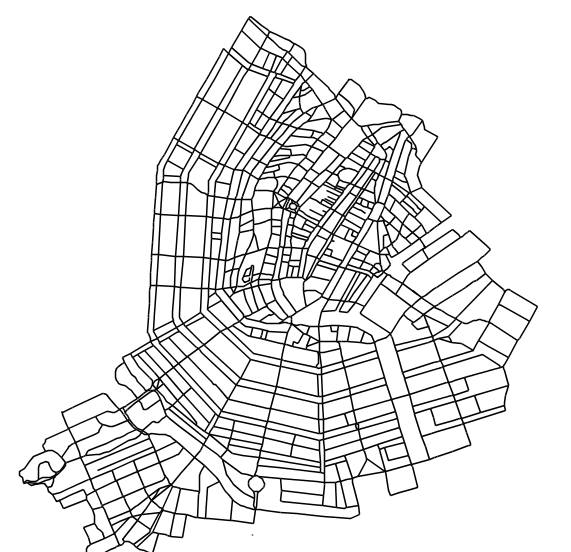
\includegraphics{images/network.png}
\caption{``Road Network''}
\end{figure}

\hypertarget{buildings}{%
\section{buildings}\label{buildings}}

This species is imported froma shapefile. The attributes of this
shapefile are imported and mapped into various model variables - as
attributes of the building species. The main classification of buildings
is based on its usage. Curerntly the model only distinguishes between
{[}office, home{]}.

\begin{figure}
\centering
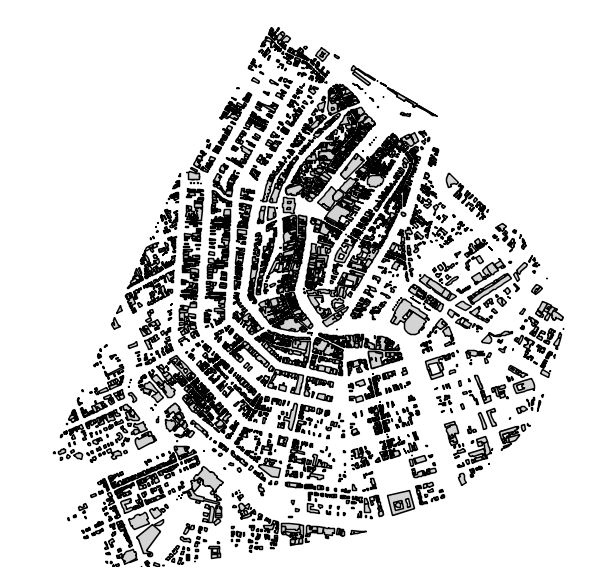
\includegraphics{images/buildings.png}
\caption{``Buildings''}
\end{figure}

\printindex


\end{document}
